% Graphic for TeX using PGF
% Title: C:\Users\Kéké\Pictures\Diagramme2.dia
% Creator: Dia v0.97.2
% CreationDate: Wed Feb 04 15:16:29 2015
% For: Kéké
% \usepackage{tikz}
% The following commands are not supported in PSTricks at present
% We define them conditionally, so when they are implemented,
% this pgf file will use them.
\ifx\du\undefined
  \newlength{\du}
\fi
\setlength{\du}{15\unitlength}
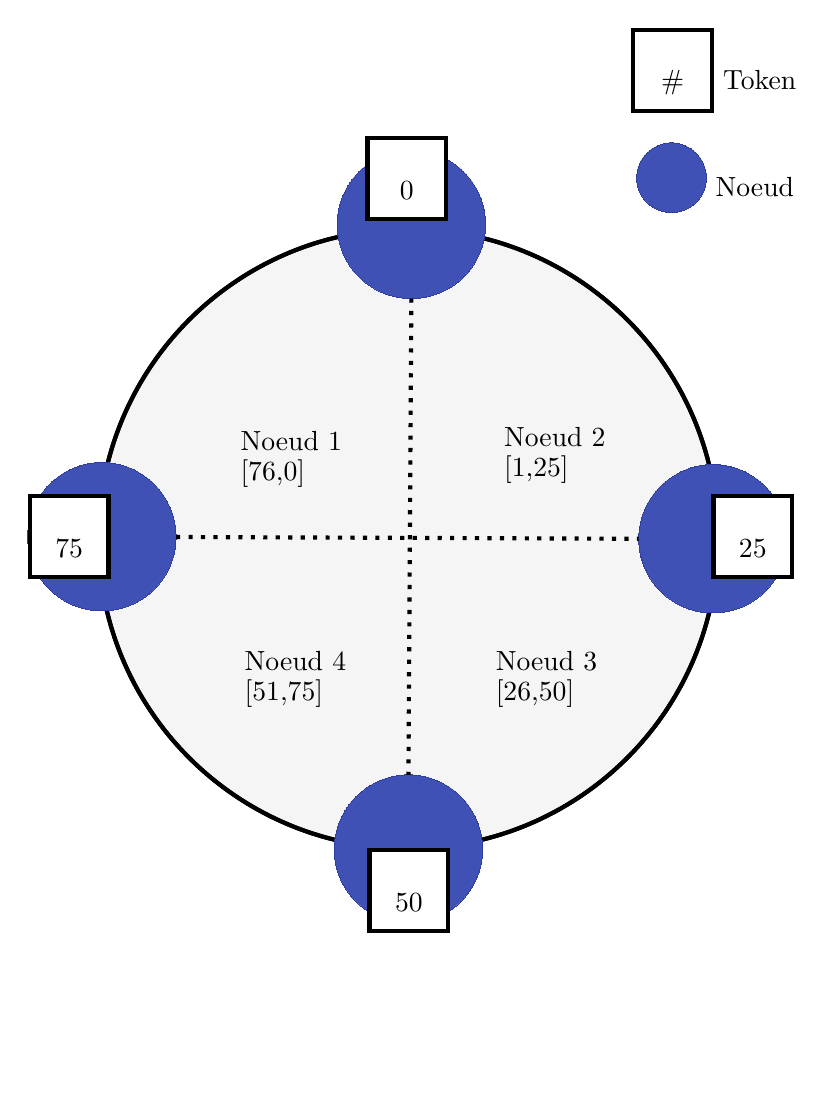
\begin{tikzpicture}
\pgftransformxscale{1.000000}
\pgftransformyscale{-1.000000}
\definecolor{dialinecolor}{rgb}{0.000000, 0.000000, 0.000000}
\pgfsetstrokecolor{dialinecolor}
\definecolor{dialinecolor}{rgb}{1.000000, 1.000000, 1.000000}
\pgfsetfillcolor{dialinecolor}
\pgfsetlinewidth{0.100000\du}
\pgfsetdash{}{0pt}
\pgfsetdash{}{0pt}
\pgfsetbuttcap
\pgfsetmiterjoin
\pgfsetlinewidth{0.100000\du}
\pgfsetbuttcap
\pgfsetmiterjoin
\pgfsetdash{}{0pt}
\definecolor{dialinecolor}{rgb}{0.960784, 0.960784, 0.960784}
\pgfsetfillcolor{dialinecolor}
\pgfpathellipse{\pgfpoint{12.662500\du}{-1.262500\du}}{\pgfpoint{7.462500\du}{0\du}}{\pgfpoint{0\du}{7.462500\du}}
\pgfusepath{fill}
\definecolor{dialinecolor}{rgb}{0.000000, 0.000000, 0.000000}
\pgfsetstrokecolor{dialinecolor}
\pgfpathellipse{\pgfpoint{12.662500\du}{-1.262500\du}}{\pgfpoint{7.462500\du}{0\du}}{\pgfpoint{0\du}{7.462500\du}}
\pgfusepath{stroke}
\pgfsetbuttcap
\pgfsetmiterjoin
\pgfsetdash{}{0pt}
\definecolor{dialinecolor}{rgb}{0.000000, 0.000000, 0.000000}
\pgfsetstrokecolor{dialinecolor}
\pgfpathellipse{\pgfpoint{12.662500\du}{-1.262500\du}}{\pgfpoint{7.462500\du}{0\du}}{\pgfpoint{0\du}{7.462500\du}}
\pgfusepath{stroke}
\pgfsetlinewidth{0.000000\du}
\pgfsetdash{}{0pt}
\pgfsetdash{}{0pt}
\pgfsetbuttcap
\pgfsetmiterjoin
\pgfsetlinewidth{0.000000\du}
\pgfsetbuttcap
\pgfsetmiterjoin
\pgfsetdash{}{0pt}
\definecolor{dialinecolor}{rgb}{0.247059, 0.317647, 0.709804}
\pgfsetfillcolor{dialinecolor}
\pgfpathellipse{\pgfpoint{12.737500\du}{-8.837500\du}}{\pgfpoint{1.787500\du}{0\du}}{\pgfpoint{0\du}{1.787500\du}}
\pgfusepath{fill}
\definecolor{dialinecolor}{rgb}{0.188235, 0.247059, 0.623529}
\pgfsetstrokecolor{dialinecolor}
\pgfpathellipse{\pgfpoint{12.737500\du}{-8.837500\du}}{\pgfpoint{1.787500\du}{0\du}}{\pgfpoint{0\du}{1.787500\du}}
\pgfusepath{stroke}
\pgfsetbuttcap
\pgfsetmiterjoin
\pgfsetdash{}{0pt}
\definecolor{dialinecolor}{rgb}{0.188235, 0.247059, 0.623529}
\pgfsetstrokecolor{dialinecolor}
\pgfpathellipse{\pgfpoint{12.737500\du}{-8.837500\du}}{\pgfpoint{1.787500\du}{0\du}}{\pgfpoint{0\du}{1.787500\du}}
\pgfusepath{stroke}
\pgfsetlinewidth{0.000000\du}
\pgfsetdash{}{0pt}
\pgfsetdash{}{0pt}
\pgfsetbuttcap
\pgfsetmiterjoin
\pgfsetlinewidth{0.000000\du}
\pgfsetbuttcap
\pgfsetmiterjoin
\pgfsetdash{}{0pt}
\definecolor{dialinecolor}{rgb}{0.247059, 0.317647, 0.709804}
\pgfsetfillcolor{dialinecolor}
\pgfpathellipse{\pgfpoint{20.002500\du}{-1.262500\du}}{\pgfpoint{1.787500\du}{0\du}}{\pgfpoint{0\du}{1.787500\du}}
\pgfusepath{fill}
\definecolor{dialinecolor}{rgb}{0.188235, 0.247059, 0.623529}
\pgfsetstrokecolor{dialinecolor}
\pgfpathellipse{\pgfpoint{20.002500\du}{-1.262500\du}}{\pgfpoint{1.787500\du}{0\du}}{\pgfpoint{0\du}{1.787500\du}}
\pgfusepath{stroke}
\pgfsetbuttcap
\pgfsetmiterjoin
\pgfsetdash{}{0pt}
\definecolor{dialinecolor}{rgb}{0.188235, 0.247059, 0.623529}
\pgfsetstrokecolor{dialinecolor}
\pgfpathellipse{\pgfpoint{20.002500\du}{-1.262500\du}}{\pgfpoint{1.787500\du}{0\du}}{\pgfpoint{0\du}{1.787500\du}}
\pgfusepath{stroke}
\pgfsetlinewidth{0.000000\du}
\pgfsetdash{}{0pt}
\pgfsetdash{}{0pt}
\pgfsetbuttcap
\pgfsetmiterjoin
\pgfsetlinewidth{0.000000\du}
\pgfsetbuttcap
\pgfsetmiterjoin
\pgfsetdash{}{0pt}
\definecolor{dialinecolor}{rgb}{0.247059, 0.317647, 0.709804}
\pgfsetfillcolor{dialinecolor}
\pgfpathellipse{\pgfpoint{12.667500\du}{6.212500\du}}{\pgfpoint{1.787500\du}{0\du}}{\pgfpoint{0\du}{1.787500\du}}
\pgfusepath{fill}
\definecolor{dialinecolor}{rgb}{0.188235, 0.247059, 0.623529}
\pgfsetstrokecolor{dialinecolor}
\pgfpathellipse{\pgfpoint{12.667500\du}{6.212500\du}}{\pgfpoint{1.787500\du}{0\du}}{\pgfpoint{0\du}{1.787500\du}}
\pgfusepath{stroke}
\pgfsetbuttcap
\pgfsetmiterjoin
\pgfsetdash{}{0pt}
\definecolor{dialinecolor}{rgb}{0.188235, 0.247059, 0.623529}
\pgfsetstrokecolor{dialinecolor}
\pgfpathellipse{\pgfpoint{12.667500\du}{6.212500\du}}{\pgfpoint{1.787500\du}{0\du}}{\pgfpoint{0\du}{1.787500\du}}
\pgfusepath{stroke}
\pgfsetlinewidth{0.000000\du}
\pgfsetdash{}{0pt}
\pgfsetdash{}{0pt}
\pgfsetbuttcap
\pgfsetmiterjoin
\pgfsetlinewidth{0.000000\du}
\pgfsetbuttcap
\pgfsetmiterjoin
\pgfsetdash{}{0pt}
\definecolor{dialinecolor}{rgb}{0.247059, 0.317647, 0.709804}
\pgfsetfillcolor{dialinecolor}
\pgfpathellipse{\pgfpoint{5.282500\du}{-1.312500\du}}{\pgfpoint{1.787500\du}{0\du}}{\pgfpoint{0\du}{1.787500\du}}
\pgfusepath{fill}
\definecolor{dialinecolor}{rgb}{0.188235, 0.247059, 0.623529}
\pgfsetstrokecolor{dialinecolor}
\pgfpathellipse{\pgfpoint{5.282500\du}{-1.312500\du}}{\pgfpoint{1.787500\du}{0\du}}{\pgfpoint{0\du}{1.787500\du}}
\pgfusepath{stroke}
\pgfsetbuttcap
\pgfsetmiterjoin
\pgfsetdash{}{0pt}
\definecolor{dialinecolor}{rgb}{0.188235, 0.247059, 0.623529}
\pgfsetstrokecolor{dialinecolor}
\pgfpathellipse{\pgfpoint{5.282500\du}{-1.312500\du}}{\pgfpoint{1.787500\du}{0\du}}{\pgfpoint{0\du}{1.787500\du}}
\pgfusepath{stroke}
\pgfsetlinewidth{0.100000\du}
\pgfsetdash{{\pgflinewidth}{0.200000\du}}{0cm}
\pgfsetdash{{\pgflinewidth}{0.200000\du}}{0cm}
\pgfsetbuttcap
{
\definecolor{dialinecolor}{rgb}{0.000000, 0.000000, 0.000000}
\pgfsetfillcolor{dialinecolor}
% was here!!!
\definecolor{dialinecolor}{rgb}{0.000000, 0.000000, 0.000000}
\pgfsetstrokecolor{dialinecolor}
\draw (12.737500\du,-7.050000\du)--(12.667500\du,4.425000\du);
}
\pgfsetlinewidth{0.100000\du}
\pgfsetdash{{\pgflinewidth}{0.200000\du}}{0cm}
\pgfsetdash{{\pgflinewidth}{0.200000\du}}{0cm}
\pgfsetbuttcap
{
\definecolor{dialinecolor}{rgb}{0.000000, 0.000000, 0.000000}
\pgfsetfillcolor{dialinecolor}
% was here!!!
\definecolor{dialinecolor}{rgb}{0.000000, 0.000000, 0.000000}
\pgfsetstrokecolor{dialinecolor}
\draw (7.069954\du,-1.305589\du)--(18.215000\du,-1.262500\du);
}
\pgfsetlinewidth{0.100000\du}
\pgfsetdash{}{0pt}
\pgfsetdash{}{0pt}
\pgfsetbuttcap
\pgfsetmiterjoin
\pgfsetlinewidth{0.100000\du}
\pgfsetbuttcap
\pgfsetmiterjoin
\pgfsetdash{}{0pt}
\definecolor{dialinecolor}{rgb}{1.000000, 1.000000, 1.000000}
\pgfsetfillcolor{dialinecolor}
\fill (11.682258\du,-10.925000\du)--(11.682258\du,-8.965000\du)--(13.579032\du,-8.965000\du)--(13.579032\du,-10.925000\du)--cycle;
\definecolor{dialinecolor}{rgb}{0.000000, 0.000000, 0.000000}
\pgfsetstrokecolor{dialinecolor}
\draw (11.682258\du,-10.925000\du)--(11.682258\du,-8.965000\du)--(13.579032\du,-8.965000\du)--(13.579032\du,-10.925000\du)--cycle;
\pgfsetbuttcap
\pgfsetmiterjoin
\pgfsetdash{}{0pt}
\definecolor{dialinecolor}{rgb}{0.000000, 0.000000, 0.000000}
\pgfsetstrokecolor{dialinecolor}
\draw (11.682258\du,-10.925000\du)--(11.682258\du,-8.965000\du)--(13.579032\du,-8.965000\du)--(13.579032\du,-10.925000\du)--cycle;
\pgfsetlinewidth{0.100000\du}
\pgfsetdash{}{0pt}
\pgfsetdash{}{0pt}
\pgfsetbuttcap
\pgfsetmiterjoin
\pgfsetlinewidth{0.100000\du}
\pgfsetbuttcap
\pgfsetmiterjoin
\pgfsetdash{}{0pt}
\definecolor{dialinecolor}{rgb}{1.000000, 1.000000, 1.000000}
\pgfsetfillcolor{dialinecolor}
\fill (20.015000\du,-2.300000\du)--(20.015000\du,-0.340000\du)--(21.911774\du,-0.340000\du)--(21.911774\du,-2.300000\du)--cycle;
\definecolor{dialinecolor}{rgb}{0.000000, 0.000000, 0.000000}
\pgfsetstrokecolor{dialinecolor}
\draw (20.015000\du,-2.300000\du)--(20.015000\du,-0.340000\du)--(21.911774\du,-0.340000\du)--(21.911774\du,-2.300000\du)--cycle;
\pgfsetbuttcap
\pgfsetmiterjoin
\pgfsetdash{}{0pt}
\definecolor{dialinecolor}{rgb}{0.000000, 0.000000, 0.000000}
\pgfsetstrokecolor{dialinecolor}
\draw (20.015000\du,-2.300000\du)--(20.015000\du,-0.340000\du)--(21.911774\du,-0.340000\du)--(21.911774\du,-2.300000\du)--cycle;
\pgfsetlinewidth{0.100000\du}
\pgfsetdash{}{0pt}
\pgfsetdash{}{0pt}
\pgfsetbuttcap
\pgfsetmiterjoin
\pgfsetlinewidth{0.100000\du}
\pgfsetbuttcap
\pgfsetmiterjoin
\pgfsetdash{}{0pt}
\definecolor{dialinecolor}{rgb}{1.000000, 1.000000, 1.000000}
\pgfsetfillcolor{dialinecolor}
\fill (11.730000\du,6.225000\du)--(11.730000\du,8.185000\du)--(13.626774\du,8.185000\du)--(13.626774\du,6.225000\du)--cycle;
\definecolor{dialinecolor}{rgb}{0.000000, 0.000000, 0.000000}
\pgfsetstrokecolor{dialinecolor}
\draw (11.730000\du,6.225000\du)--(11.730000\du,8.185000\du)--(13.626774\du,8.185000\du)--(13.626774\du,6.225000\du)--cycle;
\pgfsetbuttcap
\pgfsetmiterjoin
\pgfsetdash{}{0pt}
\definecolor{dialinecolor}{rgb}{0.000000, 0.000000, 0.000000}
\pgfsetstrokecolor{dialinecolor}
\draw (11.730000\du,6.225000\du)--(11.730000\du,8.185000\du)--(13.626774\du,8.185000\du)--(13.626774\du,6.225000\du)--cycle;
\pgfsetlinewidth{0.100000\du}
\pgfsetdash{}{0pt}
\pgfsetdash{}{0pt}
\pgfsetbuttcap
\pgfsetmiterjoin
\pgfsetlinewidth{0.100000\du}
\pgfsetbuttcap
\pgfsetmiterjoin
\pgfsetdash{}{0pt}
\definecolor{dialinecolor}{rgb}{1.000000, 1.000000, 1.000000}
\pgfsetfillcolor{dialinecolor}
\fill (3.545000\du,-2.300000\du)--(3.545000\du,-0.340000\du)--(5.441774\du,-0.340000\du)--(5.441774\du,-2.300000\du)--cycle;
\definecolor{dialinecolor}{rgb}{0.000000, 0.000000, 0.000000}
\pgfsetstrokecolor{dialinecolor}
\draw (3.545000\du,-2.300000\du)--(3.545000\du,-0.340000\du)--(5.441774\du,-0.340000\du)--(5.441774\du,-2.300000\du)--cycle;
\pgfsetbuttcap
\pgfsetmiterjoin
\pgfsetdash{}{0pt}
\definecolor{dialinecolor}{rgb}{0.000000, 0.000000, 0.000000}
\pgfsetstrokecolor{dialinecolor}
\draw (3.545000\du,-2.300000\du)--(3.545000\du,-0.340000\du)--(5.441774\du,-0.340000\du)--(5.441774\du,-2.300000\du)--cycle;
% setfont left to latex
\definecolor{dialinecolor}{rgb}{0.000000, 0.000000, 0.000000}
\pgfsetstrokecolor{dialinecolor}
\node at (12.630645\du,-9.652500\du){0};
% setfont left to latex
\definecolor{dialinecolor}{rgb}{0.000000, 0.000000, 0.000000}
\pgfsetstrokecolor{dialinecolor}
\node at (20.963387\du,-1.027500\du){25};
% setfont left to latex
\definecolor{dialinecolor}{rgb}{0.000000, 0.000000, 0.000000}
\pgfsetstrokecolor{dialinecolor}
\node at (12.678387\du,7.497500\du){50};
% setfont left to latex
\definecolor{dialinecolor}{rgb}{0.000000, 0.000000, 0.000000}
\pgfsetstrokecolor{dialinecolor}
\node at (4.493387\du,-1.027500\du){75};
% setfont left to latex
\definecolor{dialinecolor}{rgb}{0.000000, 0.000000, 0.000000}
\pgfsetstrokecolor{dialinecolor}
\node[anchor=west] at (5.350000\du,11.575000\du){};
% setfont left to latex
\definecolor{dialinecolor}{rgb}{0.000000, 0.000000, 0.000000}
\pgfsetstrokecolor{dialinecolor}
\node[anchor=west] at (14.700000\du,-3.725000\du){Noeud 2};
% setfont left to latex
\definecolor{dialinecolor}{rgb}{0.000000, 0.000000, 0.000000}
\pgfsetstrokecolor{dialinecolor}
\node[anchor=west] at (14.700000\du,-2.925000\du){\ensuremath{[}1,25\ensuremath{]}};
% setfont left to latex
\definecolor{dialinecolor}{rgb}{0.000000, 0.000000, 0.000000}
\pgfsetstrokecolor{dialinecolor}
\node[anchor=west] at (15.750000\du,-3.925000\du){};
% setfont left to latex
\definecolor{dialinecolor}{rgb}{0.000000, 0.000000, 0.000000}
\pgfsetstrokecolor{dialinecolor}
\node[anchor=west] at (14.500000\du,1.675000\du){Noeud 3};
% setfont left to latex
\definecolor{dialinecolor}{rgb}{0.000000, 0.000000, 0.000000}
\pgfsetstrokecolor{dialinecolor}
\node[anchor=west] at (14.500000\du,2.475000\du){\ensuremath{[}26,50\ensuremath{]}};
% setfont left to latex
\definecolor{dialinecolor}{rgb}{0.000000, 0.000000, 0.000000}
\pgfsetstrokecolor{dialinecolor}
\node[anchor=west] at (8.450000\du,1.675000\du){Noeud 4};
% setfont left to latex
\definecolor{dialinecolor}{rgb}{0.000000, 0.000000, 0.000000}
\pgfsetstrokecolor{dialinecolor}
\node[anchor=west] at (8.450000\du,2.475000\du){\ensuremath{[}51,75\ensuremath{]}};
% setfont left to latex
\definecolor{dialinecolor}{rgb}{0.000000, 0.000000, 0.000000}
\pgfsetstrokecolor{dialinecolor}
\node[anchor=west] at (8.350000\du,-3.625000\du){Noeud 1};
% setfont left to latex
\definecolor{dialinecolor}{rgb}{0.000000, 0.000000, 0.000000}
\pgfsetstrokecolor{dialinecolor}
\node[anchor=west] at (8.350000\du,-2.825000\du){\ensuremath{[}76,0\ensuremath{]}};
\pgfsetlinewidth{0.100000\du}
\pgfsetdash{}{0pt}
\pgfsetdash{}{0pt}
\pgfsetbuttcap
\pgfsetmiterjoin
\pgfsetlinewidth{0.100000\du}
\pgfsetbuttcap
\pgfsetmiterjoin
\pgfsetdash{}{0pt}
\definecolor{dialinecolor}{rgb}{1.000000, 1.000000, 1.000000}
\pgfsetfillcolor{dialinecolor}
\fill (18.082258\du,-13.525000\du)--(18.082258\du,-11.566667\du)--(19.977419\du,-11.566667\du)--(19.977419\du,-13.525000\du)--cycle;
\definecolor{dialinecolor}{rgb}{0.000000, 0.000000, 0.000000}
\pgfsetstrokecolor{dialinecolor}
\draw (18.082258\du,-13.525000\du)--(18.082258\du,-11.566667\du)--(19.977419\du,-11.566667\du)--(19.977419\du,-13.525000\du)--cycle;
\pgfsetbuttcap
\pgfsetmiterjoin
\pgfsetdash{}{0pt}
\definecolor{dialinecolor}{rgb}{0.000000, 0.000000, 0.000000}
\pgfsetstrokecolor{dialinecolor}
\draw (18.082258\du,-13.525000\du)--(18.082258\du,-11.566667\du)--(19.977419\du,-11.566667\du)--(19.977419\du,-13.525000\du)--cycle;
% setfont left to latex
\definecolor{dialinecolor}{rgb}{0.000000, 0.000000, 0.000000}
\pgfsetstrokecolor{dialinecolor}
\node at (19.029839\du,-12.253333\du){\#};
% setfont left to latex
\definecolor{dialinecolor}{rgb}{0.000000, 0.000000, 0.000000}
\pgfsetstrokecolor{dialinecolor}
\node[anchor=west] at (19.977419\du,-12.323333\du){Token};
\pgfsetlinewidth{0.000000\du}
\pgfsetdash{}{0pt}
\pgfsetdash{}{0pt}
\pgfsetbuttcap
\pgfsetmiterjoin
\pgfsetlinewidth{0.000000\du}
\pgfsetbuttcap
\pgfsetmiterjoin
\pgfsetdash{}{0pt}
\definecolor{dialinecolor}{rgb}{0.247059, 0.317647, 0.709804}
\pgfsetfillcolor{dialinecolor}
\pgfpathellipse{\pgfpoint{19.005000\du}{-9.960000\du}}{\pgfpoint{0.840000\du}{0\du}}{\pgfpoint{0\du}{0.840000\du}}
\pgfusepath{fill}
\definecolor{dialinecolor}{rgb}{0.188235, 0.247059, 0.623529}
\pgfsetstrokecolor{dialinecolor}
\pgfpathellipse{\pgfpoint{19.005000\du}{-9.960000\du}}{\pgfpoint{0.840000\du}{0\du}}{\pgfpoint{0\du}{0.840000\du}}
\pgfusepath{stroke}
\pgfsetbuttcap
\pgfsetmiterjoin
\pgfsetdash{}{0pt}
\definecolor{dialinecolor}{rgb}{0.188235, 0.247059, 0.623529}
\pgfsetstrokecolor{dialinecolor}
\pgfpathellipse{\pgfpoint{19.005000\du}{-9.960000\du}}{\pgfpoint{0.840000\du}{0\du}}{\pgfpoint{0\du}{0.840000\du}}
\pgfusepath{stroke}
% setfont left to latex
\definecolor{dialinecolor}{rgb}{0.000000, 0.000000, 0.000000}
\pgfsetstrokecolor{dialinecolor}
\node[anchor=west] at (19.845000\du,-9.737500\du){Noeud};
\end{tikzpicture}
